\chapter{Proteomics study}
\label{ch:proteomics}

\section{Introduction}

Under the impulse of \jyoti, \james\ has reprocessed \enquote{more diverse}
large-scale \ms-based proteomic studies on normal human tissues to this day.

See \Cref{sec:ProteoData} for more details about the details of the datasets and
the pipeline.

See \Cref{subsec:distribPlot} and more particularly \Cref{fig:densityCutler_log2,%
fig:densityKuster_log2,fig:densityPandey_log2}

After exploring the transcriptomic side (way more data) I have explored the
proteomic (\ms-based) before integrating the trancriptomic to the proteomic.
It seems to be the obvious/sensible thing to do.

\begin{figure}[htpb]
    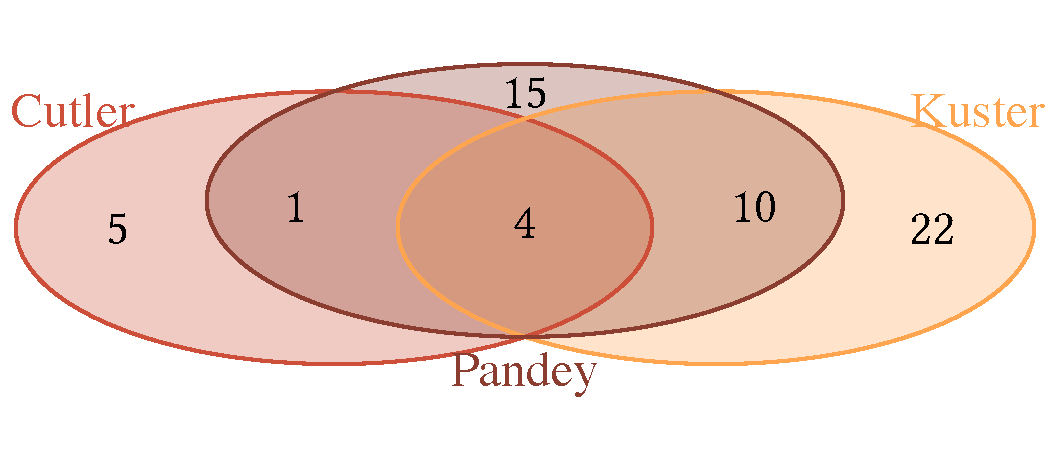
\includegraphics[scale=1]{proteomics/VennDiagProtCond.pdf}\centering
    \caption[ ]{\label{VennDiagProt3}\textbf{<++>}<++>}
\end{figure}

\section{Results}

\subsection{Limited availability (and overlap) of tissues}

\subsection{Disparate universe: High-throughput proteomics has a greater
variability of detection and quantification than high-throughput transcriptomics}

It is more about identification than quantification.

\subsection{About half of the quantified proteins for a given tissue are found
in different datasets}

\subsection{Technical variability seems to prevail over biological signal:
correlations between samples from a same tissue are globally lesser than
correlation between samples from a same study.}


\section{Discussion}


%%%% Maybe?
%%%Quantification with the first method
%%%Quantification with the second method with PPKM
%%%%
